

\documentclass{beamer}
% Theme choice:
\usetheme{Warsaw}

% Want to be able to cite, without printing bibliography
\usepackage{bibentry}
\usepackage[backend=bibtex,style=authoryear]{biblatex}
\addbibresource{ImaiKeane.bib}



% But set a Boolean so I can omit the TOC before the intro


% This sets up a Boolean variable which will allow us to display the TOC at the beginning of each section, with the specific section in bold, while omitting this step when we want to. 


\RequirePackage{ifthen} % package required
\newboolean{sectiontoc}
\setboolean{sectiontoc}{true} % default to true

\AtBeginSection[]
{
  \ifthenelse{\boolean{sectiontoc}}{
    \begin{frame}
      \frametitle{Table of Contents}
      \tableofcontents[currentsection]
    \end{frame}
  }
}

\newcommand{\toclesssection}[1]{
  \setboolean{sectiontoc}{false}
  \section{#1}
  \setboolean{sectiontoc}{true}
}


\usepackage{tikz}

\title{INTERTEMPORAL LABOR SUPPLY AND HUMAN CAPITAL ACCUMULATION}

\author{SUSUMU IMAI AND MICHAEL P. KEANE}

\date{December 2000}


\begin{document}


\frame{\titlepage}


\toclesssection{Introduction and Motivation}
\begin{frame}
  \frametitle{Intertemporal elasticity of substitution in labor supply}
  \begin{itemize}
  \item This has long been an area of study, see \cite{Lucas1969-ti}
  %\item Studies using micropanel data in structural models include \cite{MaCurdy1981-iy}, \cite{Browning1985-ox}, and \cite{Altonji1986-zf}.
  \item Are unable to solve a puzzle: although wages grow throughout the life cycle, hours worked do not
    \begin{itemize}
    \item Why don't workers work less when young and wages are low and more when they are old and wages are high?
      \end{itemize}
  \end{itemize}
\end{frame}

\begin{frame}
  \frametitle{Human capital}
  \begin{itemize}
  \item The answer: wages are determined by human capital which grows with work experience
  \item Workers face competing motivations: wages grow through the life cycle, but returns to human capital decrease
        \begin{itemize}
        \item The result is a relatively flat labor supply (see next slide)
        \end{itemize}
  \item Previous research which does not account for human capital thus underestimates the elasticity of labor supply
  \end{itemize}
\end{frame}

\begin{frame}
 \frametitle{Life cycle path}
% Drawing figure 1, illustration of life cycle labor supply
%\hypertarget{OptimalSupply}
\begin{figure}[tbp]
 \centerline{
  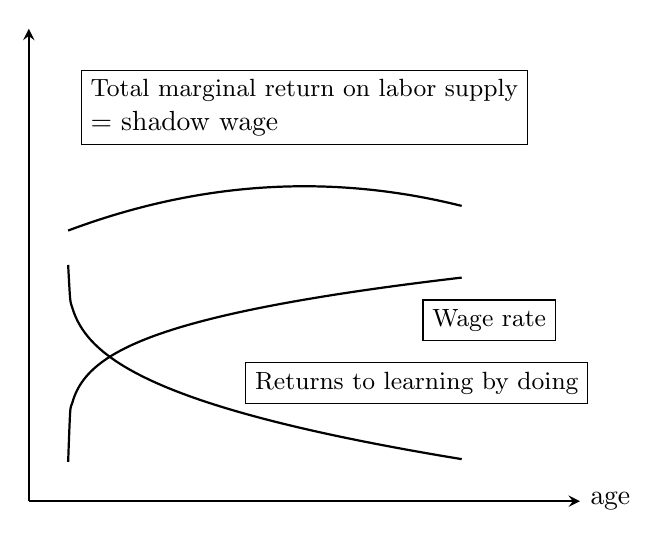
\begin{tikzpicture}
\draw[-stealth, black, thick] (0,0) -- (7,0) node[right] { age};
\draw[-stealth, black, thick] (0,0) -- (0,6);
\draw[thick, smooth, samples=200, xshift=.5cm, yshift=.5cm, domain=0:5] plot ({ \x, {(6*\x)^(1/4)}});
\node[right] at (5,2.3) [rectangle,draw] {\small Wage rate};
\draw[thick, smooth, samples=200, xshift=.5cm, yshift=3cm, domain=0:5] plot ({ \x, {-(3*\x)^(1/3)}});
\node[right] at (2.75,1.5) [rectangle,draw] {\small Returns to learning by doing};
% \draw[thick, smooth, samples=200, xshift=.5cm, yshift=2.5cm, domain=0.05:2.05] plot ({ \x, {\x^(1/2)-\x^(1/3)}});
\draw[thick, smooth, samples=200, xshift=-.5cm, yshift=2cm, domain=1:6] plot ({ \x, {2-(\x/4 - 1)^2}});
\node[align=left] at (3.5,5) [rectangle,draw] {\small Total marginal return on labor supply \\ = shadow wage};
\end{tikzpicture}
}
\caption{OPTIMAL LIFE CYCLE LABOR SUPPLY}
\label{fig:OptimalSupply}
\end{figure}
\end{frame}

\begin{frame}
  \frametitle{Table of Contents}
  \tableofcontents
\end{frame}
    
    \section{Model}
    \begin{frame}
      \frametitle{}
      \begin{figure}[H]
        \centering
      %  \includegraphics[height=0.8\textheight]{}
      \end{figure}
  \end{frame}

 
    \section{Solution}
    \begin{frame}
      \frametitle{}
      \begin{itemize}
        \item 
        \item
        \item
        \item
        \end{itemize}
  \end{frame}
  
  \section{Data}
  \begin{frame}
    \frametitle{}
      \begin{itemize}
      \item 
      \item 
      \item 
    \end{itemize}
  \end{frame}

  \section{Summary and Conclusion}

   \begin{frame}
    \frametitle{}
    \begin{enumerate}
    \item 
    \item
    \item
    \end{enumerate}
  \end{frame}

 % \nobibliography{./ImaiKeane.bib}
  
\end{document}